\documentclass[./examen.tex]{subfiles}

\begin{document}
\begin{center}
\makebox[\textwidth]{Nombre y Apellido:\enspace\hrulefill}
\end{center}
\begin{multicols}{2}
\begin{questions}
 \question Un electroimán tiene una Fuerza de $F=100Kg$ y su inducción magnética en el hierro es de $B=2T$.
 \begin{parts}
    \part[2] Calcular la sección del electroimán $S$ en $cm^2$ y calcular la intensidad de campo magnético $H$ si la permeabilidad relativa del núcleo de electroimán es $\mu_r=7000$
 \end{parts}
\question El circuito de la figura está construído de chapa magnética $\mu_r=200$, se desea una inducción de $B=2T$ la bobina es de $N=2000$ espiras.  
\begin{parts}
\part[2] Calcular la longitud de la línea media $l_m$ en metros. 
\part[2] Calcular la Intensidad de campo en el núcleo $H$ en $Av/m$.
\part[2] Fuerza magnetomotriz $\mathscr{F}$ amperios-vuelta necesarios.
\part[2] Intensidad de corriente que circula por la bobina.
\end{parts}
\end{questions}
\columnbreak
\centering
  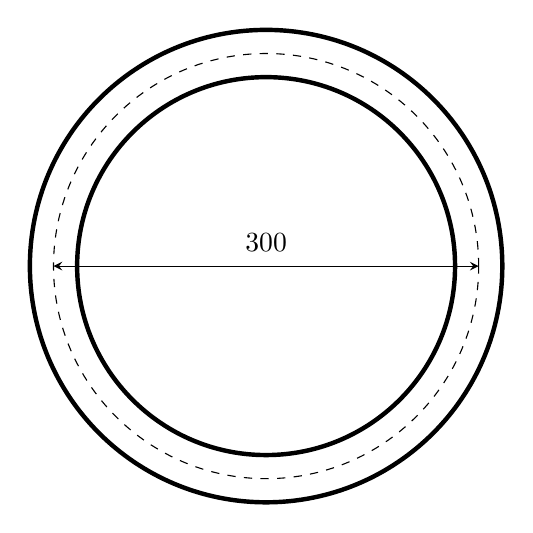
\begin{tikzpicture}[scale=0.03]
    \draw [dashed, thin] (0,0) circle [radius=90];
    \draw [ultra thick] (0,0) circle [radius=100];
    \draw [ultra thick] (0,0) circle [radius=80];
    \draw [stealth-stealth] (-90,0)--(90,0);
    \draw (0,10) node[]{300};
    \end{tikzpicture}

\end{multicols}




 \end{document}